In this chapter, we first explain graph OLAP with real examples. Then we briefly introduce Neo4j, a state-of-art graph database system, which is employed as the back end of our proposed solution. In addition, we review and summarize the most recent relevant works on graph OLAP processing.


%----------------------------------------------------------------------
\section{OLAP over Property Graph Model}
%----------------------------------------------------------------------


As noted in the previous chapter, in the property graph model, each node and edge could have arbitrary number and type of properties. A type of property is represented as follows:

\begin{displaymath}
\centering
[NodeType].[PropertyType]
\end{displaymath}

For example, User.Age denotes an ``Age'' attribute associated with a node of type ``User''. In order to identify a node or edge, a unique ID is assigned to each node and edge. For simplicity, in this thesis we represent IDs of nodes or edges of a certain type as ID([NodeType]) or ID([EdgeType]). For example, ID(User) refers to unique IDs of ``User'' nodes. Note that in some scenarios, a unique ID can be considered as a special kind of property for its corresponding node or edge.


OLAP (On-Line Analytical Processing) \cite{DBLP:conf/sigmod/BeyerR99, DBLP:journals/datamine/GrayCBLRVPP97, DBLP:conf/sigmod/ZhaoDN97} usually employs a cube concept, which is constructed over multiple attributes, in order to provide users a multi-dimensional and multi-level view for effective data analysis from different perspectives and with multiple granularities. The key operations in an OLAP framework are slice/dice and roll-up/drill-down, with slice/dice focusing on a particular aspect of the data, roll-up performing generalization if users only want to see a concise overview, and drill-down performing specialization if more details are needed. We shall detail the cube technique from the graph data perspective later in this chapter.


%The ``graph'' in our work refers to property graphs. As introduced in Section 1.1, property graph is more flexible and powerful than classic attribute graphs.

\subsection{Graph OLAP Examples}
\label{OLAPExamples}
Graph OLAP was first proposed by Graph Cube \cite{DBLP:conf/sigmod/ZhaoLXH11} to refer to OLAP over graphs, although no formal definition of the notion Graph OLAP was given. In order to better elaborate how ``Graph OLAP'' is interpreted in this thesis, consider the following four example scenarios, where we perform OLAP queries over the StackExchange graph.

\noindent\textbf{Example 1} Does the number of high upvotes of a user indicate a high-quality post?

\fbox{
	Query \#1: Get average post score grouped by user’s upvotes.
}

Sample query result:
\begin {center}
\begin{tabular}{ l l }
	User.UpVotes&AVG(Post.Score)\\\hline
	0&1.33\\
	1&2.23\\
	2&2.34\\
	3&2.77\\
	4&3.43\\\hline
\end{tabular}
\end {center}

From the query result we can see that upvotes can be used as a good indicator of a user's post quality. Suppose we would like to propose suggested posts based on scores. When a post is freshly posted and the score of the post has not been voted, we may use the author’s upvotes as a factor to estimate the quality of his or her post.

\noindent\textbf{Example 2} Following the context of Query \#1, but this time we want to take a closer look at how  upvotes are correlated with post scores for different types of posts. It is reasonable to guess that authors' upvotes make more difference in scores of their answers (posts with PostTypeId 2) than their questions (posts with PostTypeId 1), because a user's level of expertise is usually better reflected by his or her answers.

\fbox{
	Query \#2:  Get average post score grouped by user’s upvotes and post’s post types.
}

Sample query result:

\begin {center}
\begin{tabular}{ l l l }
	User.Upvotes&Post.PostTypeId&AVG(Post.Score)\\\hline
	0&1&2.14\\
	1&1&2.26\\
	2&1&2.83\\
	3&1&3.04\\
	4&1&3.46\\
	0&2&1.54\\
	1&2&2.21\\
	2&2&2.18\\
	3&2&2.72\\
	4&2&3.58\\\hline
\end{tabular}
\end {center}

The query results reveal that users with higher upvotes not only provide good answers but ask valuable questions as well. However, there is a subtle difference on how upvotes are correlated with scores of questions and answers. For example, a really low upvote level indicates a low-quality answer more than a low-quality question. This is probably because people tend to be tolerant of a naive question rather than with a wrong answer.

Query \#1 and Query \#2 simply focus on relationship between User and Post. We may switch our attention to a slightly more complicated structure by adding the Tag.

\noindent\textbf{Example 3} In year 2017, what is the weighted average age of users? For instance is ‘python’ more trendy than ‘c’ among young users?

\fbox{
	Query \#3: For each tag, get the weighted average age of users who have posted posts on the tag in 2017. In other words, we group all the posts that were posted in 2017 by their tag names and calculate the weighted average users' age under each tag.
}

Sample query result:

\begin {center}
\begin{tabular}{ l l  }
	
	TagName&AVG(Age)\\\hline
	Router&19.6\\
	Python&24.1\\
	Internet&26.8\\
	C&30.2\\
	programmer&31.4\\
	software&29.8\\\hline
	
\end{tabular}
\end {center}

From the results, one can tell the average users' age with respect to each tag clearly and easily compares them. It reveals some interesting insights. We know that Python may have a relatively young user group, compared with C. Similarly, ``Router'' is a topic that is more often discussed among youngsters than the general topic of ``Internet''. Note that we are led to the above findings based on the recent posts (posted in year 2017).

%\noindent\textbf{Example 4} Following Query \#3, for each tag, find out the trend of weighted average users' age by years. 
%
%\fbox{
%Query \#4: Get average user age grouped by tags and years of creation of the posts.
%}
%
%Sample query result:
%
%\begin {center}
%\begin{tabular}{ l l  l}
%	
%	TagName & Year & AVG(Age) \\\hline
%	Router & 2012 & 22.1 \\
%	Router & 2017 & 19.6 \\
%	Python & 2012 & 27.3 \\
%	Python & 2017 & 24.1 \\
%	Internet & 2012 & 27.5 \\
%	Internet & 2017 & 26.8 \\
%	C & 2012 & 30.4 \\
%	C & 2017 & 30.2 \\
%	programmer	& 2012 & 34.2 \\
%	programmer	& 2017 & 31.4 \\
%	software	& 2012 & 31.6 \\
%	software	& 2017 & 29.8\\\hline
%	
%\end{tabular}
%\end {center}
%
%We see that Trend of younger age on IT topics is revealed from the results. Python is getting faster embraced by younger people compared with C. Similarly we can compare two commercial products’ customer targeting strategy, advertising performance etc.

From the above OLAP query examples we can see that OLAP over property gra0phs provides an interactive and informative way to analyze property graphs from multiple dimensions, and thus helps people find the hidden correlations, aggregated effects, regularities, tendencies and so on.

\subsection{Structure, Dimension, and Measure}
\label{Structure, Dimension, and Measure}

We now explain the three key elements of a graph OLAP: \textit{structure}, \textit{dimension}, and \textit{measure}  using Query \#1 as an example.

%\textbf{Query \#1: 		Get average post score grouped by user’s upvotes. }

Query \#1 concerns the structure (colored in blue) shown in Figure \ref{fig:2:1}.

\begin{figure}[H]
	\centering
	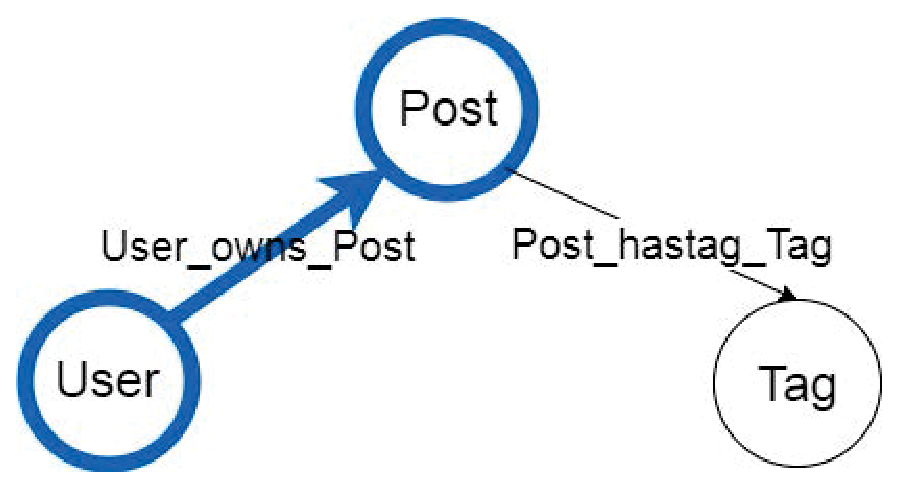
\includegraphics[scale=0.5]{pic/meta1.eps}
	\caption{\textit{Structure} of Query \#1}
	\label{fig:2:1}
\end{figure}



We say that (User)-[User\_owns\_post]-$>$(Post) is the structure of Query \#1. The query is first aggregated on users' upvotes. We say that {User.Upvotes} is the dimension of Query \#1, and the output of the query is an aggregation function on post’s score.  We say that {AVG(Post.Score)} is the measure of Query \#1. Similarly, consider Example 2, which shares the same structure as shown in Figure \ref{fig:2:1}. The dimensions of Query \#2 is {User.Upvotes, Post.PostTypeId}, and the measure is {AVG(Post.Score)}. Note that Query \#2 adds Post.PostTypeId to Query \#1’s dimensions. In other words, Query \#2 asks for a more detailed partitions over dimensions. We call Query \#2 a drill-down from Query \#1, and  Query \#1 is a roll-up from Query \#2. Note that possible property combinations can be modeled as a lattice-structured cube. Figure \ref{fig:2:2} shows what a cube is like for properties \{A,B,C\}. We can see that roll-up and drill-down operations allow us to navigate up and down on a cube.


\begin{figure}[H]
	\centering
	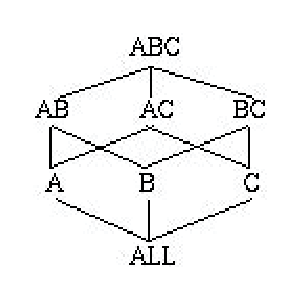
\includegraphics[scale=1]{pic/22.eps}
	\caption{Cube of properties \{A,B,C\}.}
	\label{fig:2:2}
\end{figure}

\textbf{Query \#3: 		Get average user age grouped by users’ 2017 posts’ tags.}

Structure:	(User)-[User\_owns\_post]-(Post)-[Post\_hastag\_Tag]-(Tag)
\begin{figure}[H]
	\centering
	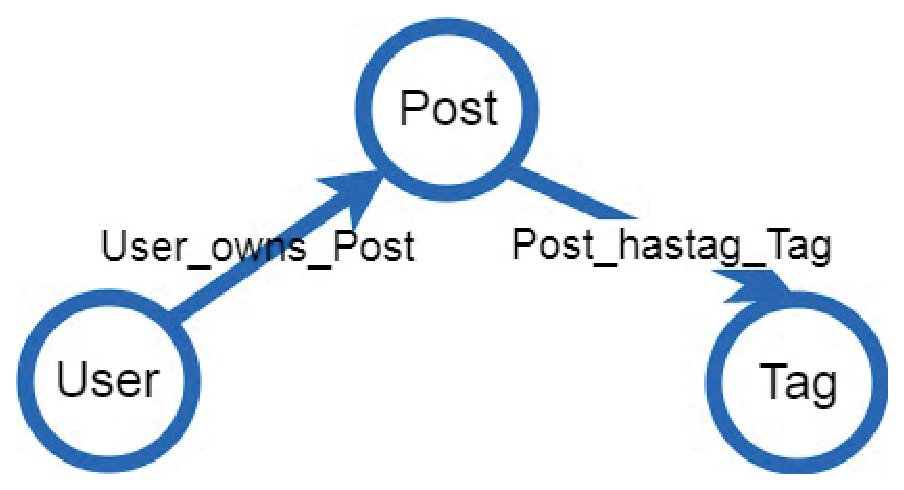
\includegraphics[scale=0.5]{pic/meta2.eps}
	\caption{\textit{Structure} of Query \#3}
	\label{fig:2:3}
\end{figure}


Dimensions:	{Tag.Tagname}

Measure:	{AVG(User.Age)}

Note that Query \#3 has a different \textit{structure} than Query \#1 and Query \#2, as shown in Figure \ref{fig:2:3}. Query \#3 enforces a requirement that post must be created in year 2017, which picks out a particular subset of  the posts. In OLAP this is called ``slicing'' operation. Slicing operation allows users to view the data with constraints on selected properties. In this thesis we call these constraints (e.g., \{Post.Year=2017\} in Query \#3) \textit{``slicing conditions''}.

To summarize, graph OLAP allows clients to aggregate different \textit{structures}, over different \textit{dimensions}, on different \textit{measures}, and optionally slice aggregation result by different \textit{slicing conditions}. Clients can change their views by performing roll-up, drill-down, and slicing freely and interactively.


%----------------------------------------------------------------------
\section{Graph Databases and Neo4j}
%----------------------------------------------------------------------
Emerging online applications concerning graph processing has motivated the relational database community to support efficient graph management \cite{DBLP:conf/grades/Xirogiannopoulos17} \cite{DBLP:conf/bigdataconf/JindalMCH15}. However, there has been active debate about the efficiency of using traditional RDBMS for graph computing considering the unique query workload against graph data~\cite{DBLP:conf/edbt/HolschSG17} \cite{DBLP:journals/corr/JoishiS17}. Relational and graph database systems both have their own strengths in term of query processing. In this thesis, we work with graph database systems.

%There are two major types of databases that store and process graph data: traditional relational databases and graph databases.

%Relational databases  model graph data as entity and relationship tables. For example, given a simple property graph shown in Figure \ref{fig:2:4}, which consists of 1 user and 3 posts, a relational database stores the graph with 3 tables:
%
%\begin{figure}[H]
%\centering
%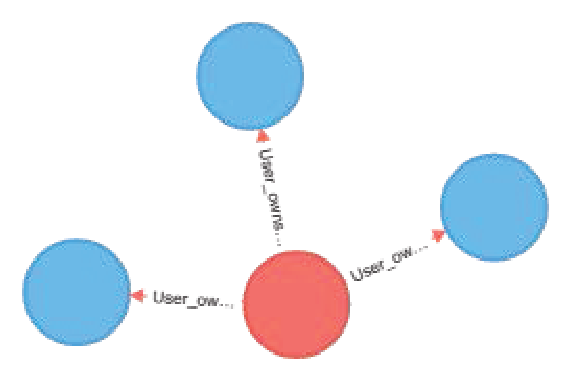
\includegraphics[scale=0.9]{pic/4.eps}
%\caption{A simple property graph.}
%\label{fig:2:4}
%\end{figure}
%
%
%\begin{center}
%\begin{tabular}{|c|c|c| }
%	\hline
%	\multicolumn{3}{|c|}{User} \\\hline
%	Uid	& Age & UpVote	\\ \hline
%	1 & 22 & 5 \\\hline
%\end{tabular}
%\end {center}
%
%
%\begin{center}
%	\begin{tabular}{|c|c|}
%	\hline
%	\multicolumn{2}{|c|}{Post} \\\hline
%		Pid	& Score	\\ \hline
%		1	& 0.5 \\
%		2	& 0.8 \\
%		3	& 0.6 \\\hline
%	\end{tabular}
%	\end {center}	
%
%
%\begin{center}
%	\begin{tabular}{|c|c|}
%	\hline
%	\multicolumn{2}{|c|}{Owns} \\\hline
%		Uid	& Pid	\\ \hline
%		1	&1 \\
%		1	&2 \\
%		1	&3 \\\hline
%	\end{tabular}
%	\end {center}


%There are two drawbacks of storing property graphs in a relational database. First, each node or edge in a property graph could have arbitrary types of properties. However, relational table schema would restrict nodes or edges of the same type to have a uniform set of properties (attributes). Second and more importantly, edges are stored as a separate table in relational databases. Thus, we cannot directly query all the posts of a given user without joining User and Own tables in the above example.

In graph databases, the storage structure that is most commonly used in an adjacency list. An adjacency list is a list that stores all the edges and neighbor nodes for a given node. A popular graph database system is Neo4j. Like most traditional RDBMS, Neo4j holds atomicity, consistency, isolation and durability (ACID). Neo4j's native graph processing engine enables SQL like queries over property graphs which are managed by its own graph storage. Common features in RDBMS such as indexes building and constraints are also supported. REST API plus official drivers for programming languages such as Java are provided for the sake of easy interactions with other programs. One most special feature about Neo4j is that it allows multiple-labeled nodes and edges; for example, a node referring to a male student could have various labels such as ``student'' and ``male'' and etc.

Cypher, Neo4j's query language, is a powerful SQL like query language, which is expressive and simple. For example, consider the following query: what is the average score group by different user upvotes when PostTypeID is 2? A Cypher query would be written as follows:

\begin{verbatim}
match (u:User)-[r:User\_owns\_Post]-$>$(p:Post)
where p.PostTypeId=`2'
return u.Upvotes, AVG(p.Score)
\end{verbatim}

In the above Cypher query, ``User'' and ``Post'' are node labels, PostTypeId and Score are properties of ``Post'', ``UpVotes'' is a property of ``User''.

%Neo4j is written in Java. While applications in various languages could interact the server by issuing queries and transport using BOLT protocol. BOLT protocol is a binary protocol implemented by Neo4j team. It is more efficient than HTTP protocol.

%Figure 2.4 shows how applications interact with Neo4j server.
%
%\begin {figure}[H]
%\centering
%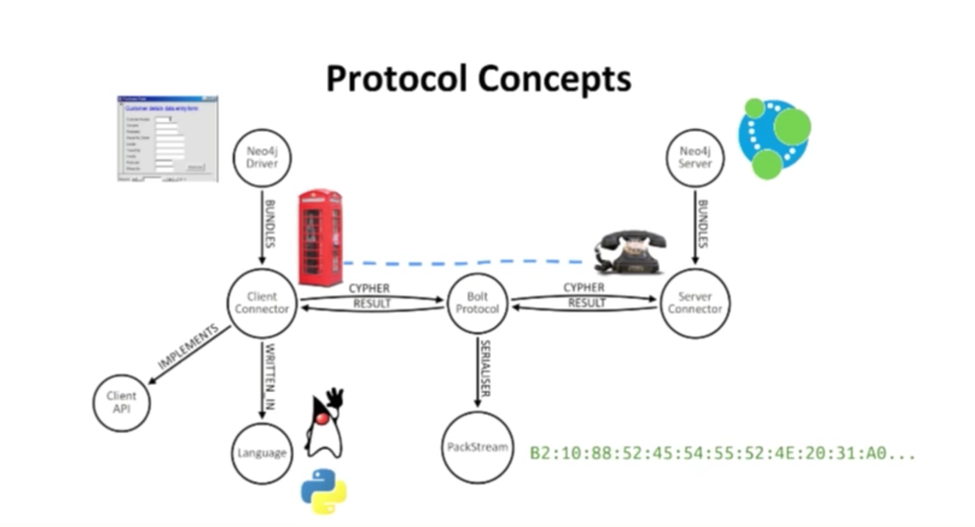
\includegraphics[scale=0.4]{pic/23.png}
%\caption{How applications interact with Neo4j server.}
%\end{figure}


%----------------------------------------------------------------------
\section{Related Work}
%----------------------------------------------------------------------



There have been a few work discussing efficient graph OLAP queries on attribute graphs or RDF graphs.

Cube-based \cite{DBLP:conf/sofsem/JakawatFL16} proposes the concept of  graphs enriched by cubes. Each node and edge of the considered network are described by a cube. It allows the user to quickly analyze the information summarized into cubes. It works well in slowly changing dimension problem in OLAP analysis.

Gagg \cite{DBLP:conf/esws/MaaliCD15} introduces an RDF graph aggregation operator that is both expressive and flexible. It defines its operational semantics on top of SPARQL algebra, and proposes an algorithm to answer graph aggregation queries. Gagg achieves significant improvements in performance compared to plain-SPARQL graph aggregation.

Pagrol \cite{DBLP:conf/icde/WangFWTAA14} provides an efficient MapReduce-based parallel graph cubing algorithm, MRGraph-Cubing, to compute the graph cube for an attributed graph.

Graph Cube \cite{DBLP:conf/sigmod/ZhaoLXH11} introduces a data warehousing model that supports OLAP queries effectively on large multidimensional networks. It takes account of both attribute aggregation and structure summarization of the networks. In order to deal with ``curse of dimensions'', a greedy algorithm framework is introduced for partial materialization of cuboids. Moreover, it addresses and defines two most important notions in graph OLAP scenarios as \textit{dimension} and \textit{measure}. Note that in our work, \textit{structure} (of meta graph) is addressed as a third important notion (as discussed in \ref{Structure, Dimension, and Measure}). Graph Cube \cite{DBLP:conf/sigmod/ZhaoLXH11} focuses on OLAP senerios over a fixed \textit{structure}, with \textit{dimension} and \textit{measure} varied, whereas our work deals with OLAP workloads over various \textit{structures}. %Graph Cube \cite{DBLP:conf/sigmod/ZhaoLXH11} views the outcome of Graph OLAP as aggregated graphs (aggregation of data graph). On the contrary, in our work, we consider the outcome of Graph OLAP as results of OLAP queries.

Graph OLAP \cite{DBLP:conf/icdm/ChenYZHY08} studies dimensions and measures in the graph OLAP scenario and furthermore develops a conceptual framework for data cubes on graphs. It differentiates different types of measures (e.g., distributive measures and holistic measures) by their properties during aggregation. It looks into different semantics of OLAP operations, and classifies the framework into two major subcases: informational OLAP and topological OLAP. It points out a graph cube can be fully or partially materialized by calculating a special kind of measure called aggregated graph.

In Graph Cube \cite{DBLP:conf/sigmod/ZhaoLXH11}, concepts of graph cube is introduced. Given a particular structure S, a property set P, and measure set M. We can aggregate over S on $2^{|P|}$ different combinations of dimensions. These $2^{|P|}$ queries can be mapped as a lattice structure, where each combination of dimensions corresponds to a cuboid in the lattice. We call the lattice structure of these $2^{|P|}$ queries a graph cube.


It has been pointed out in  Graph OLAP \cite{DBLP:conf/icdm/ChenYZHY08} that as long as the domain of measure is a subset of \{COUNT, SUM, AVERAGE\} and M contains COUNT(*), the following feature holds: given any two cuboids $C_1$ and $C_2$ from the same graph cube, as long as dimension($C_2$) is a subset of dimension($C_1$), result of $C_1$ can be used to generate result of $C_2$. This means that once a cuboid is materialized, all roll-up operations from this cuboid could be processed simply by scanning the materialized cuboid result. This will dramatically decrease roll-up operation time compared to aggregation from data graph (often of larger size, disk I/O), scanning materialized cuboid result (often of smaller size) is often much faster.


Ideally we can materialize all cuboids. But when the number of dimension is large, number of cuboids grows exponentially, making total materialization hard due to overwhelming space cost. To solve this Graph Cube \cite{DBLP:conf/sigmod/ZhaoLXH11} proposed a partial materialization algorithm on graph cube. It is a greedy algorithm and the score function is based on benefits of deduction of total computation cost.

\begin{table}
	\footnotesize
	\begin{center}
		\begin{tabular}{ | c | c | c | c | c |  }
			\hline
			& G. Type & Q. Pattern & Layered & Featuer\\ \hline
			Cube-based \cite{DBLP:conf/sofsem/JakawatFL16} & Property & Simple relation & yes & Cubes on edges and nodes\\ \hline
			Gagg \cite{DBLP:conf/esws/MaaliCD15} & Property & Exact match & no & Structural patterns\\ \hline
			Pagrol \cite{DBLP:conf/icde/WangFWTAA14} & Property & edge \& node attributes & yes & Map-Reduce computing\\ \hline
			Graph Cube \cite{DBLP:conf/sigmod/ZhaoLXH11} & Homogenous  & node attributes & yes & Partial materialization\\ \hline
			Graph OLAP \cite{DBLP:conf/icdm/ChenYZHY08} & Property & edge \& node attributes & yes & Distributive and holistic measures\\ \hline
			
		\end{tabular}
		\end {center}
		\caption{A summary of graph OLAP literature}
	\end{table}
	
	
	From the summary, we categorize the existing work into two lines. The first focuses on a simple subset of property graphs (e.g., graphs with only homogenous nodes and edges), and proposes optimizations in order to accelerate OLAP query processing (e.g., Graph Cube \cite{DBLP:conf/sigmod/ZhaoLXH11}). Although attribute-aware optimizations are proposed in some literature, structure-aware optimizations are not studied. Second focuses on a relatively high-level framework that processes generic queries over generic property graphs (e.g., Gagg \cite{DBLP:conf/esws/MaaliCD15}). However, query processing efficiency is not the main focus.
	
	To conclude, there is not enough study on structure-aware optimizations for efficient graph OLAP. As mentioned in Section 1.3, efficiency issue is one of the most challenging issues on graph OLAP. Therefore, we investigate faster structure-aware OLAP processing over general property graphs.
	
	
	
	%----------------------------------------------------------------------
	%\section{Graph Cube}
	%----------------------------------------------------------------------
	
	
